\subsection*{\textbf{Задание 12.5} Решение уравнений и системы уравнений.}
Решите уравнение $x^4 + x^3 - 5x - 12 = 0$;
решите системы уравнений двумя сопособами, используя функции \textbf{Solve} и \textbf{LinearSolve} от переменных $x$, $y$.
\[
    \begin{cases}
        ax + by = c \\
        sx + fy = h \\
    \end{cases}
\]

\begin{figure}[H]
    \renewcommand{\figurename}{Рисунок}
    \centering{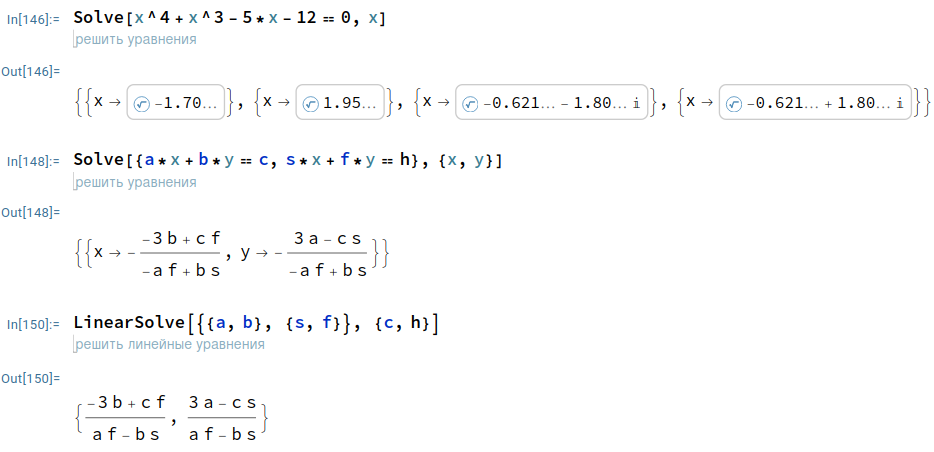
\includegraphics[scale=0.50]{body/img/12_5.png}}
    \label{fig:image_12_5}
\end{figure}